\chapter{INTRODUCCIÓN}\label{cap:Introduccción}
%\markboth{\thechapter. Introducción}{\thechapter. Introducción}

\section{Motivación}
\lhead[\thepage]{Sección \thesection. Motivación}

Los manipuladores paralelos son sistemas mecánicos diseñados como una serie de enlaces conectados por junturas accionadas por motor. Estas junturas generalmente son actuadores lineales denominados como brazos móviles, que se extienden desde una base fija a una plataforma superior sostenida. El movimiento sincronizado de estos brazos móviles permite realizar distintas elevaciones, rotaciones y movimientos de la plataforma dependiendo de la longitud de cada brazo. El hecho de estar conectados a una base fija, los brazos otorgan la firmeza necesaria del movimiento hacia la plataforma superior.

Estos manipuladores paralelos son frecuentemente ocupados en simuladores de alta fidelidad para modelar distintos movimientos y desplazamientos \cite{anderson2004hexapods,wang2010perfomancemanipulators,merlet1992ParallelMS}.  Generalmente, estos tipos de manipuladores proveen una mayor precisión, mayor rigidez, mayor relación de carga-peso y proporcionan una mejor distribución de la carga que otros tipos de manipuladores. 

Existen distintos tipos de manipuladores con diferentes grados de libertad (DOFs) dependiendo del objetivo buscado, tales como el robot tipo DELTA \cite{pierrot1990deltarobot} de $3$ DOFs, el HEXA robot \cite{pierrot1991hexarobot} de $6$ DOFs o el manipulador paralelo más popular llamado plataforma Gough-Stewart \cite{stewart1965} de $6$ DOFs. Es posible apreciar en la Figura \ref{fig:StewartPlatform} el tipo de manipulador paralelo de $6$ brazos identificado como plataforma Stewart.

Los manipuladores de $6$ DOFs mencionados son los más utilizados al otorgar una mayor cantidad de movimientos y rotaciones complejas en comparación a sus versiones más simples con menores grados de libertad. Es por esto que el diseño de control de estos manipuladores posee un grado de dificultad por todas las interacciones que posee. A través del tiempo se han estudiado muchos diseños de control para plataformas de $6$ DOFs, los cuales han avanzado en complejidad a través de los años con los nuevos avances tecnológicos que han surgido. El diseño de control más común utilizado en la plataforma Stewart es el control proporcional integral derivativo (PID), que en ocasiones ha sido optimizado mediante algoritmos computacionales para obtener mejoras en el desempeño. En la mayoría de estos casos el control PID posee una estructura descentralizada, es decir, una estructura diagonal de controladores de una entrada y una salida (SISO). Sin embargo, no existe en la literatura un contraste con la versión de múltiples entradas y múltiples salidas (MIMO) del PID, es decir, con los elementos fuera de la diagonal de sus matrices distintos de cero (MIMO PID full). Debido a esto es posible plantear la siguiente pregunta ¿será significativa la mejora en el desempeño al cambiar de un control PID descentralizado a un MIMO PID full en una plataforma Stewart?. Esto motiva a realizar una comparación del desempeño entre ambos controladores, con el fin de determinar en qué casos es más conveniente utilizar el PID MIMO full o el PID descentralizado, dependiendo de su aplicación.

Por otro lado, el área del seguimiento de señales sinusoidales en los manipuladores paralelos tampoco ha sido ampliamente desarrollado. Casi toda la gama de los tipos de control estudiados en la plataforma Stewart carecen de un diseño especializado en el seguimiento sinusoidal en estado estacionario. Si el objetivo general siempre es tener un buen desempeño del control, ¿es posible diseñar un control con seguimiento perfecto a sinusoides para la plataforma Stewart, tanto para sinusoidales de igual frecuencia como de distinta frecuencia?. Con un controlador diseñado especialmente para seguir a sinusoides de distintas características (amplitud, frecuencia y fase) se lograría un seguimiento más efectivo que beneficiaria el uso de estos manipuladores en áreas que se requieran de una aplicación más detallada. Esto lleva a la segunda motivación de la Tesis que consiste en estudiar distintos diseños de control para el seguimiento de señales sinusoidales de la plataforma Stewart. La principal contribución consiste en lograr un diseño de control que garantice un seguimiento eficiente en estado estacionario a distintas señales sinusoidales como referencia. En el marco de este análisis, el diseño de control se propone personalizable para cada brazo actuador al considerar una señal sinusoidal especifica en cada brazo, diferenciándose en amplitud, frecuencia y fase entre señales sinusoidales. 

\begin{figure}[ht]
    \centering
    \begin{subfigure}[b]{0.45\textwidth}
        \centering
        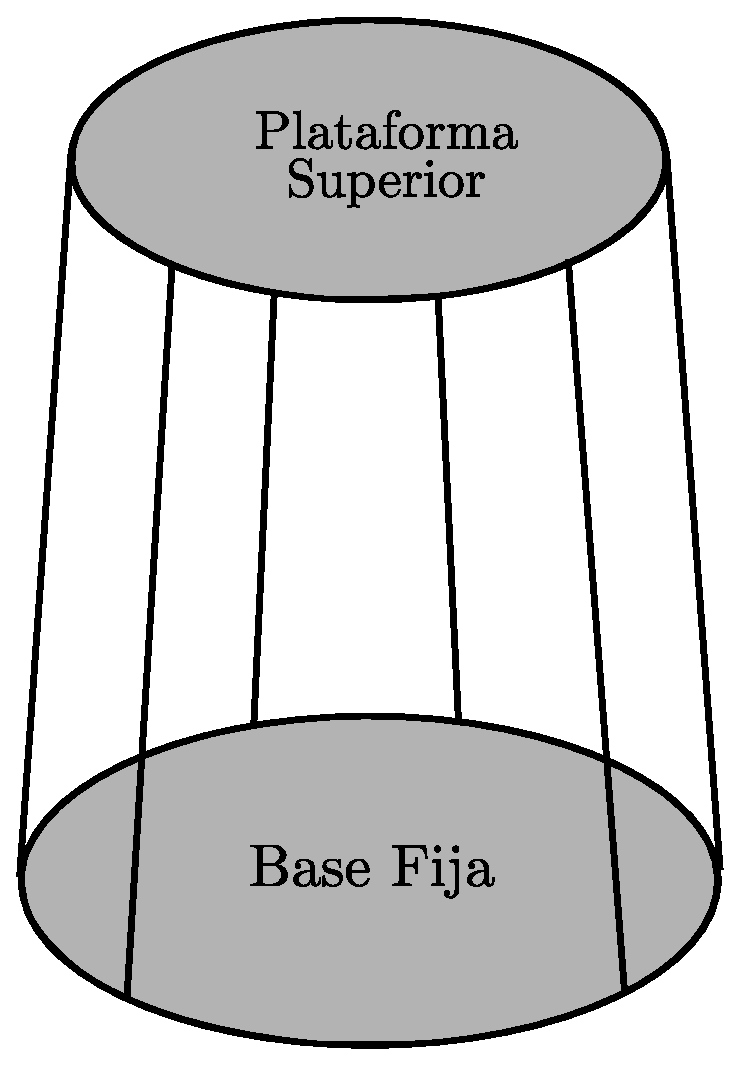
\includegraphics[width=0.5\columnwidth]{Figures/stewart1.eps}
        \caption{Esquema Plataforma Stewart}
        \label{fig:stewart1}
    \end{subfigure}
    \hfill
    \begin{subfigure}[b]{0.45\textwidth}
       \centering
        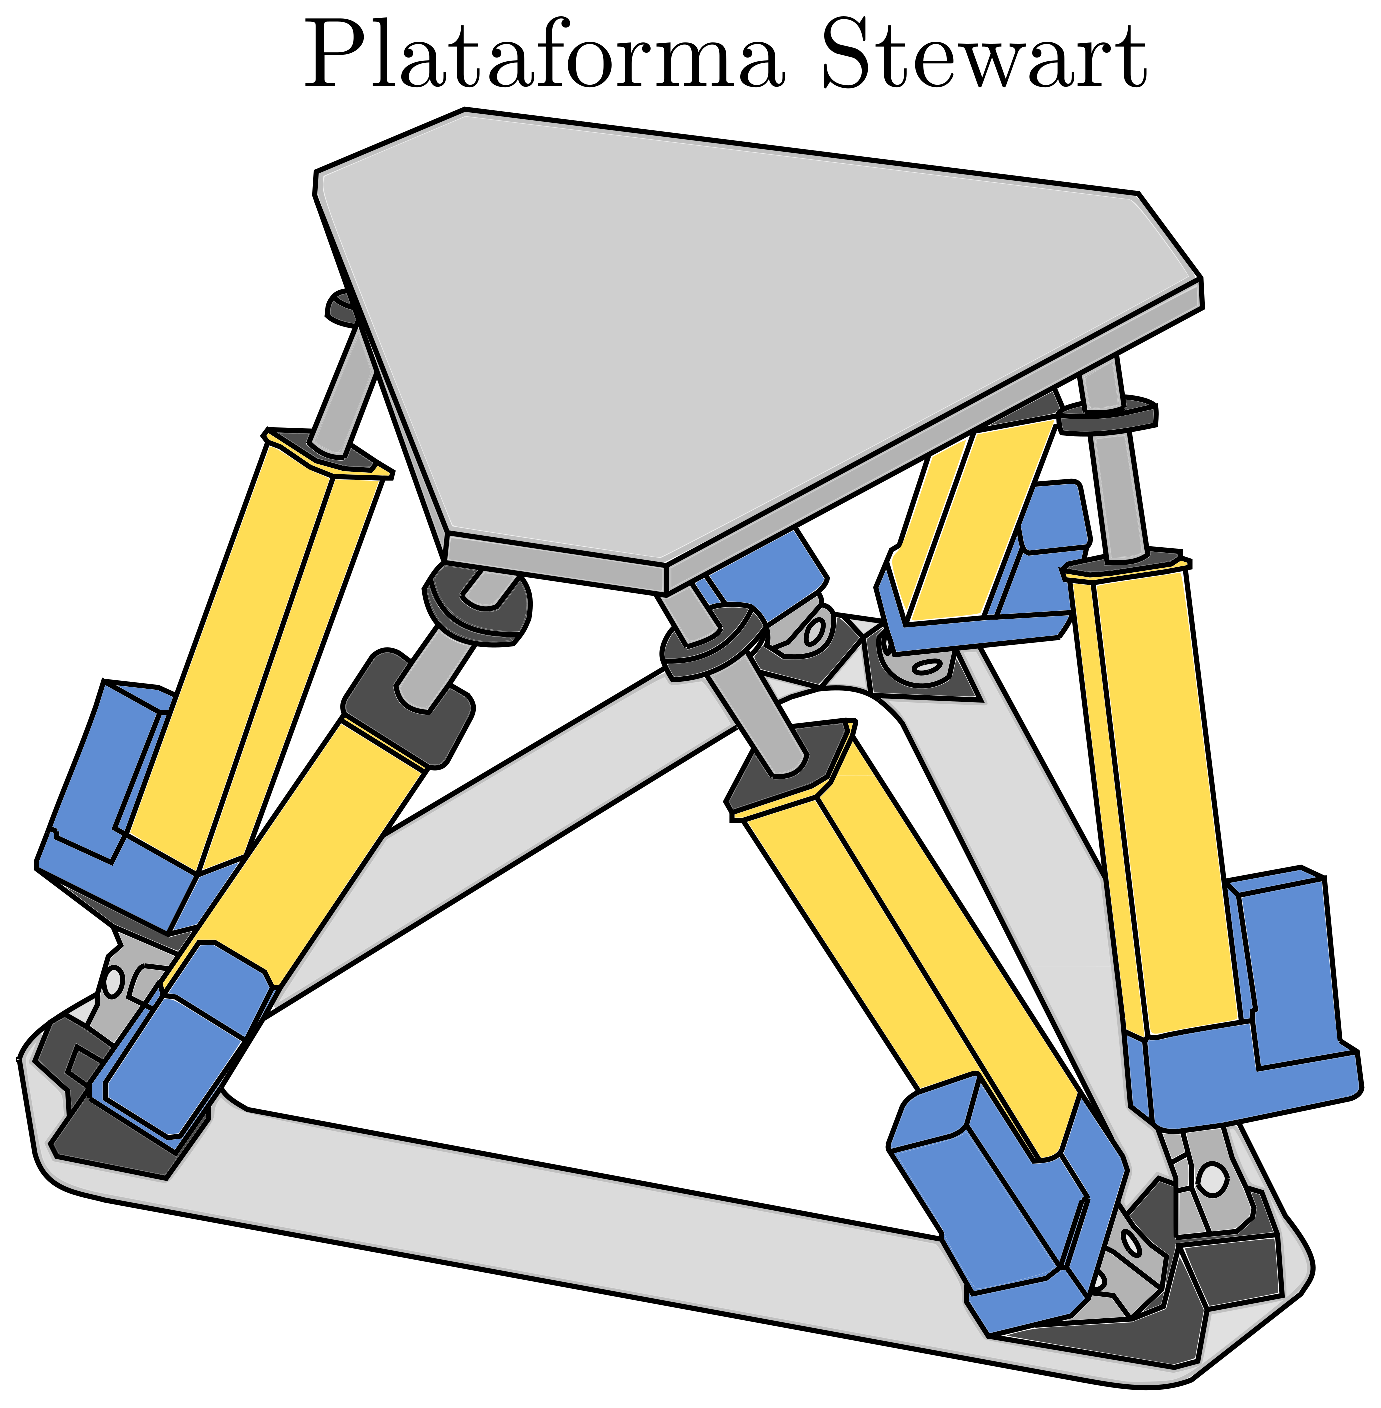
\includegraphics[width=0.7\columnwidth]{Figures/stewart3.eps}
        \caption{Plataforma Stewart}
        \label{fig:stewart2}
    \end{subfigure}
   \caption{Plataforma Stewart}
   \label{fig:StewartPlatform}
\end{figure}






\section{Estado del arte}
\lhead[\thepage]{Sección \thesection. Estado del arte}

Una plataforma Stewart es un sistema mecánico diseñado para poder manipular la posición (movimiento lateral, longitudinal y vertical) y orientación (pitch, roll \& yaw) de una plataforma sostenida en paralelo a una base de montaje fija. Dicha plataforma es manipulada a través de actuadores lineales cuyos extremos son fijados en ambas plataformas mediante junturas móviles. La configuración más común de una plataforma Stewart comprende de 6 actuadores lineales, como se aprecia en la Figura \ref{fig:StewartPlatform}, brindando así soporte y precisión al movimiento buscado.

Este tipo de manipulador paralelo de 6 DOFs se desarrolló en 1965 por \textit{Stewart} \cite{stewart1965} para simulaciones de vuelo, siendo conocida así como la plataforma Stewart. También es conocido como Gough-platform quien presentó su uso práctico del sistema \cite{stewart1965}.
\textit{Earl and Rooney} \cite{earl1983kinematicMD} analizaron la estructura cinemática para aplicaciones robóticas y sus interconexiones en serie y paralelas.  
En \cite{do1988InverseDA} usaron el método Newton-Euler para resolver la dinámica inversa de la plataforma Stewart, en ausencia de fricción en las articulaciones y brazos. 
Por otro lado, en \cite{geng1992} se desarrollaron las ecuaciones de movimiento de Lagrange relacionadas con la geometría y distribución de inercia del manipulador.

Este sistema es utilizado actualmente en diversas aplicaciones debido a la versatilidad en el movimiento que posee, tales como sistemas de posicionamiento de antenas/radares y paneles solares \cite{lin2006disturbance,keshtkar2016adaptive}, aplicaciones en la medicina \cite{boian2004dual,girone2001stewart}, simuladores de vuelo en tiempo real \cite{pradipta2013development, huang2017incremental}, plataforma ball and plate \cite{bang2018ballandplate,kassem2015ballandplatecomparison}, etc. 

Debido a la gran cantidad de grados de libertad que posee junto a su no linealidad, conlleva a ser un sistema complejo de controlar de forma eficiente. La dinámica de la plataforma suele ser simulada en distintas investigaciones con distintos software de simulación como Matlab o ADAMS \cite{tajdari2021discrete,liu2023fuzzy}, ya que brindan un mejor modelado al considerar distintas restricciones tales como colisión de objetos, rigidez y elasticidad de cuerpos rígidos, fricción entre superficies, etc. 

Muchos autores han estudiado la formulación del modelo dinámico y su simulación de forma detallada \cite{bingul2012modeling}, además de distintos diseños de control tales como control predictivo basado en modelos (MPC) \cite{nadimi2006model}, control de modo deslizante (SMC) \cite{jouini2013modeling,chalanga2015smooth}, regulador cuadrático lineal (LQR) \cite{rossell2015tracking}, control integral cuadrático lineal (LQI) \cite{tajdari2021discrete}, entre otros. Sin embargo, el control más común es el proporcional integral derivativo (PID) \cite{liu2023fuzzy,yang2008modeling,csumnu2017motor}, que en la mayoría de los casos posee una estructura descentralizada, es decir, el controlador es una matriz diagonal de controladores PID de una entrada y una salida \cite{astrom19951pidcontrollers,skogestad2005multivariable}.
Los análisis anteriores de los controladores PID se basan en la obtención de las constantes proporcional, integral y derivativa, así como se realiza en \cite{liu2023fuzzy} mediante un diseño de control difuso (Fuzzy), o como en \cite{silva2006lqr} mediante un control LQR y LQI para sistemas mecánicos generales. Todos estos diseños de control han demostrado un aumento en la efectividad y eficiencia del control de la plataforma Stewart, sin embargo son controles descentralizados \cite{albertos2006multivariable} y además para seguimiento de señales tipo escalón como referencia. Al ser controles descentralizados, es decir con estructura diagonal de controladores SISO, consideran inexistente la interacción entre los distintos actuadores, facilitando la implementación considerablemente. Sin embargo, el diseño de un controlador MIMO PID full, es decir, una matriz de controladores PID con todos sus elementos distintos de cero en general \cite{albertos2006multivariable}, si consideraría las interacciones entre los distintos actuadores pudiendo así mejorar el desempeño del control. Este tipo de control MIMO PID full no ha sido reportado en la literatura para el control de este tipo de plataformas.

Para lograr un mejor rendimiento en el control, es posible ocupar métodos numéricos de optimización para los controladores. Distintos autores han utilizado diferentes formas de optimización tales como en \cite{choubey2021optimized} utilizando un \textit{squirrel search algorithm}, en \cite{tajdari2021optimizer} mediante una red neuronal artificial o en \cite{silva2006lqr} donde se utiliza un algoritmo numérico de optimización. Estos algoritmos demuestran una mejora significativa en los tipos de control, logrando un mejor seguimiento de las señales de referencia. En el caso de un controlador MIMO PID, utilizar estos algoritmos en las versiones descentralizadas mejorarían significativamente su desempeño, optimizando los controladores comúnmente utilizados en este tipo de plataforma por la mayoría de los autores.

Por otro lado, en el ámbito de seguimiento de señales sinusoidales, se han estudiado las limitaciones del rendimiento de sistemas lineales multivariables en el seguimiento de referencias sinusoidales en \cite{su2003performance,su2005performance,su2009performance}. Se analizan distintos casos de disponibilidad de datos de la referencia al controlador, para determinar la influencia directa del acceso a la información en el rendimiento. Se demuestra que el rendimiento solo depende de la frecuencia de la referencia sinusoidal y de la interacción entre la referencia con los ceros de fase no mínima del sistema. Las expresiones obtenidas muestran la degradación del rendimiento según la información parcial disponible de la referencia sinusoidal. Sin embargo, el estudio del seguimiento de señales sinusoidales sobre esta plataforma no es un área muy explorada. En \cite{lin2003sinusoidal} se enfocan en un esquema adaptativo de cancelación de perturbaciones sinusoidales mediante algoritmos de diseño de tolerancia a fallos (\textit{fault tolerant pointing algorithms}). Este diseño es capaz de realizar un seguimiento en baja frecuencia, rechazar grandes perturbaciones monótonas a frecuencia media y aislar vibraciones pasivas de alta frecuencia.  

Debido a que la plataforma brinda una versatilidad de movimientos gracias a sus 6 grados de libertad, se da la posibilidad que las señales de cada actuador posean distintas frecuencias (asumiendo movimientos sinusoidales), es por esto que, poder garantizar un controlador que permita asignar la frecuencia que necesita cada actuador a cada componente del controlador MIMO, representaría una mejora significativa para este sistema. Con esto se lograría un rendimiento eficiente individualizado de cada actuador mediante un solo controlador MIMO, para distintos tipos de señales de referencia como escalones o sinusoidales. Este tipo de problema de seguimiento sinusoidal para distintas frecuencias no ha sido estudiado directamente en la plataforma Stewart. Para la resolución de este problema, es posible desarrollar un seguimiento a señales de referencia sinusoidales en base a un diseño de control LQR para sistemas generales según \cite{lin1996outputregulation,yan2016outputregulation,huang2004bookoutputregulation}. Basado en el principio del modelo interno, este tipo de control garantiza un seguimiento óptimo de la referencia sinusoidal en estado estacionario. Debido a esto, el enfoque de la investigación radica en la obtención de un controlador MIMO para la plataforma Stewart, tal que garantice un seguimiento eficiente en estado estacionario de señales de referencia sinusoidales de distinta frecuencia, desarrollando así un control estabilizante para cada actuador del sistema multivariable.


\section{Principales contribuciones}
\lhead[\thepage]{Sección \thesection. Principales contribuciones}

%Esta tesis tiene como objetivo diseñar un control multivariable para la plataforma Stewart, tal que posea mejor desempeño que las versiones descentralizadas del control MIMO y a sus variantes optimizadas mediante algoritmos numéricos. Además, se busca diseñar un control que garantice un seguimiento eficiente en estado estacionario de señales de tipo sinusoidales de distinta frecuencia en la referencia. \\

Las dos principales contribuciones de esta Tesis se pueden resumir de la siguiente manera:
\begin{enumerate}
    \item Se propone un diseño de controlador MIMO PID full sintetizado en base a un control LQI. El desempeño de este controlador se compara con versiones descentralizadas del mismo controlador MIMO PID, así como con versiones optimizadas de los controladores descentralizados mediante un algoritmo numérico basado en un descenso del gradiente simple. Las simulaciones son desarrolladas mediante el programa Matlab Simulink por Simscape, especialmente diseñado para este tipo de plataformas multivariables, ya que incluye complejas interacciones internas de la parte mecánica y dinámica del sistema, facilitando una simulación más real de la plataforma. Los resultados obtenidos son en base a referencias de tipo escalón y sinusoidal, logrando un análisis completo de los distintos tipos de movimientos que es posible otorgar a la plataforma Stewart. Se ha demostrado que el control es eficiente para señales de tipo escalón, pero no para señales sinusoidales.
    
    \item A base de lo anterior, se propone un nuevo tipo de control que logra garantizar un seguimiento eficiente en estado estacionario para señales de referencia de tipo sinusoidal de distintas frecuencias para sistemas lineales. Para esto, mediante el concepto de Output Regulation basado en el principio del modelo interno se obtiene el controlador buscado de la plataforma Stewart. El controlador se diseña en base a un control LQR, que estabiliza las dinámicas internas de la plataforma, permitiendo el seguimiento sinusoidal de la referencia al utilizar información de la misma en el diseño del controlador. Se ilustran simulaciones de los resultados junto a un análisis comparativo con los diseños de control anteriores.
    
\end{enumerate}


\section{Publicaciones asociadas}
\lhead[\thepage]{Sección \thesection. Publicaciones asociadas}

Los principales trabajos asociados a esta Tesis son:
\begin{itemize}
    \item \textbf{Título del artículo:} Control of a Stewart platform using a MIMO PID controller. \\
        \textbf{Autores:} Tomás E. Bernal, Marco A. Gordon, Francisco J. Vargas, Alejandro A. Pacheco. \\
        \textbf{Publicado en:} Conferencia Andescon 2024.
    \item \textbf{Título del artículo:} Step and Sinusoidal Tracking Techniques for Stewart Platforms \\ 
        \textbf{Autores:} Tomás E. Bernal, Marco A. Gordon, Francisco J. Vargas, Alejandro A. Pacheco. \\
        \textbf{Estado:} En desarrollo para Revista. 
\end{itemize}

\section{Organización de la Tesis}
\lhead[\thepage]{Sección \thesection. Organización de la tesis}

La presente Tesis se organiza mediante capítulos ordenados de la siguiente manera:
\begin{itemize}
    \item  En el Capítulo \ref{cap:Notación y preliminares} se detallan definiciones y notaciones importantes para el desarrollo de la Tesis. 
    \item El Capítulo \ref{cap:modeladoStewart} tiene por objetivo desarrollar el modelado de la plataforma Stewart, ecuaciones dinámicas y linealización del sistema.
    \item En el Capítulo \ref{cap:mimoPID} se diseña el control PID MIMO full de la plataforma. Además, se analiza el desempeño del controlador con versiones descentralizadas y optimizadas del mismo.
    \item En el Capítulo \ref{cap:OutputRegulation} se diseña un nuevo tipo de control de la plataforma Stewart que garantiza un seguimiento eficiente en estado estacionario para señales de referencia de tipo sinusoidal de distintas frecuencias. 
    \item Finalmente en el Capítulo \ref{cap:Conclusiones} se mencionan las conclusiones y posibles trabajos futuros.
\end{itemize}
